The package \texttt{view.execution} holds the \texttt{\lnk{Executor}}, which adapts a \texttt{\hyperref[type:edu.kit.wavelength.client.model.ExecutionEngine]{ExecutionEngine}}.
This adaption is necessary because the reduction of a lambda term is concurrent with the UI interaction itself. 
As GWT runs in a single threaded browser environment, it has its own concurrency mechanism: A \texttt{Scheduler} that allows one to schedule a specific action at the end of the event loop of the browser.
As a result of this the Executor schedules one reduction step at the end of every event loop iteration and provides methods to control this concurrent execution.
The package also contains an \texttt{\lnk{ExecutionObserver}}, which is used by the \texttt{\lnk{Executor}} to push reduced terms that are intended to be displayed in the \texttt{\pkglnk{view}} to observers observing it.

\begin{figure}[H]
	\centering
	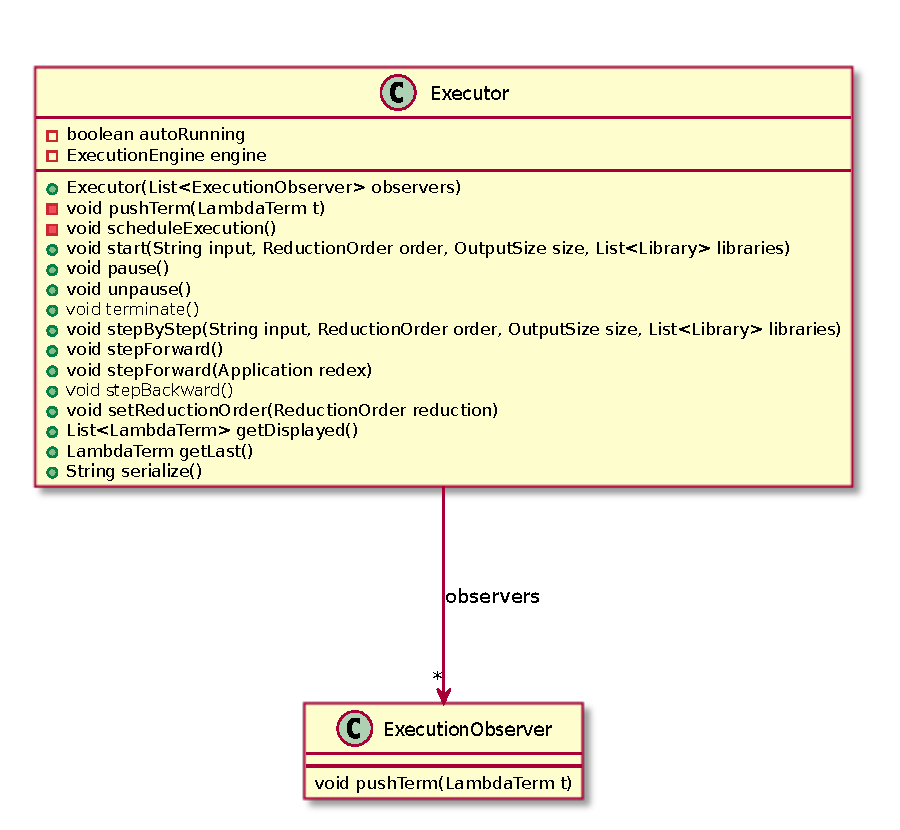
\includegraphics[width=\textwidth]{packageDiagrams/executionPackage}
\end{figure}
